\documentclass[acmlarge]{acmart}

\usepackage{booktabs} % For formal tables


\usepackage[ruled]{algorithm2e} % For algorithms
\renewcommand{\algorithmcfname}{ALGORITHM}
\SetAlFnt{\small}
\SetAlCapFnt{\small}
\SetAlCapNameFnt{\small}
\SetAlCapHSkip{0pt}
\IncMargin{-\parindent}

% Metadata Information
\acmYear{2017}
\acmMonth{7}


%\acmBadgeR[http://ctuning.org/ae/ppopp2016.html]{ae-logo}
%\acmBadgeL[http://ctuning.org/ae/ppopp2016.html]{ae-logo}


% Copyright
%\setcopyright{acmcopyright}
%\setcopyright{acmlicensed}
%\setcopyright{rightsretained}
%\setcopyright{usgov}
%\setcopyright{usgovmixed}
%\setcopyright{cagov}
%\setcopyright{cagovmixed}


% Document starts
\begin{document}
% Title portion
\title{A systematical Approach on Regulating and Reducing E-Waste.} % TODO: more precise title 
%\acmConference[SPWAL SS17]{Seminar und Praktikum "Wissenschaftliches Arbeiten und Lehren" Sommersemester 2017}{\today}{Munich, Germany} 

% Author
\author{Anita Baier}
\affiliation{\institution{Ludwigs-Maximilian-Universit\"at}
  \city{Munich} \country{Germany}}
\email{anita.baier@gmx.de} 

\author{Zhe Li}
\affiliation{\institution{Ludwigs-Maximilian-Universit\"at}
  \city{Munich} \country{Germany}}
\email{li.zhe@campus.lmu.de} 

\author{Jonas Mattes}
\affiliation{\institution{Ludwigs-Maximilian-Universit\"at}
  \city{Munich} \country{Germany}}
\email{j.mattes@campus.lmu.de} 

\author{Bruno M\"uller}
\affiliation{\institution{Ludwigs-Maximilian-Universit\"at}
  \city{Munich} \country{Germany}}
\email{muellerbr@cip.ifi.lmu.de} 

\author{An Tien Go}
\affiliation{\institution{Ludwigs-Maximilian-Universit\"at}
  \city{Munich} \country{Germany}}
\email{antiengo@campus.lmu.de}

\author{Changkum Ou}
\affiliation{\institution{Ludwigs-Maximilian-Universit\"at}
  \city{Munich} \country{Germany}}
\email{hi@changkun.us} 

\author{Guoliang Xue}
\affiliation{\institution{Ludwigs-Maximilian-Universit\"at}
  \city{Munich} \country{Germany}}
\email{guoliang.xue@campus.lmu.de} 




\begin{abstract}
\input{abstract.txt}
\end{abstract}


%
% The code below should be generated by the tool at
% http://dl.acm.org/ccs.cfm
% Please copy and paste the code instead of the example below. 
%

\ccsdesc[500]{Hardware~Power and energy}
\ccsdesc[300]{Hardware~Impact on the environment}

%
% End generated code
%


\keywords{E-waste; Fee-Upon-Disposal Regulation; Recycling.}


\maketitle

% The default list of authors is too long for headers}
\renewcommand{\shortauthors}{A. Baier et al.}

% this is just for formatting reference
%
\section{Introduction}


As a new technology, Wireless Sensor Networks (WSNs) has a wide
range of applications \cite{Culler-01, Bahl-02, Akyildiz-01}, including
environment monitoring, smart buildings, medical care, industrial and
military applications. Among them, a recent trend is to develop
commercial sensor networks that require pervasive sensing of both
environment and human beings, for example, assisted living
\cite{Akyildiz-02, Harvard-01,CROSSBOW} and smart homes
\cite{Harvard-01, Adya-01,CROSSBOW}.
% quote
\begin{quote}
  ``For these applications, sensor devices are incorporated into human
  cloths \cite{Natarajan-01, Zhou-06, Bahl-02, Adya-01} for monitoring
  health related information like EKG readings, fall detection, and
  voice recognition''.
\end{quote}
While collecting all these multimedia information
\cite{Akyildiz-02} requires a high network throughput, off-the-shelf
sensor devices only provide very limited bandwidth in a single
channel: 19.2\,Kbps in MICA2 \cite{Bahl-02} and 250\,Kbps in MICAz.

In this article, we propose MMSN, abbreviation for Multifrequency
Media access control for wireless Sensor Networks. The main
contributions of this work can be summarized as follows.
% itemize
\begin{itemize}
\item To the best of our knowledge, the MMSN protocol is the first
multifrequency MAC protocol especially designed for WSNs, in which
each device is equipped with a single radio transceiver and
the MAC layer packet size is very small.
\item Instead of using pairwise RTS/CTS frequency negotiation
\cite{Adya-01, Culler-01, Tzamaloukas-01, Zhou-06},
we propose lightweight frequency assignments, which are good choices
for many deployed comparatively static WSNs.
\item We develop new toggle transmission and snooping techniques to
enable a single radio transceiver in a sensor device to achieve
scalable performance, avoiding the nonscalable ``one
control channel + multiple data channels'' design \cite{Natarajan-01}.
\end{itemize}

% Head 1
\section{MMSN Protocol}

% Head 2
\subsection{Frequency Assignment}

We propose a suboptimal distribution to be used by each node, which is
easy to compute and does not depend on the number of competing
nodes. A natural candidate is an increasing geometric sequence, in
which
% Numbered Equation
\begin{equation}
\label{eqn:01}
P(t)=\frac{b^{\frac{t+1}{T+1}}-b^{\frac{t}{T+1}}}{b-1},
\end{equation}
where $t=0,{\ldots}\,,T$, and $b$ is a number greater than $1$.

In our algorithm, we use the suboptimal approach for simplicity and
generality. We need to make the distribution of the selected back-off
time slice at each node conform to what is shown in
Equation~\eqref{eqn:01}. It is implemented as follows: First, a random
variable $\alpha$ with a uniform distribution within the interval $(0,
1)$ is generated on each node, then time slice $i$ is selected
according to the following equation:
% Unnumbered Equation
\[
i=\lfloor(T+1)\log_b[\alpha(b-1)+1]\rfloor.
\]
It can be easily proven that the distribution of $i$ conforms to Equation
(\ref{eqn:01}).

So protocols \cite{Bahl-02, Culler-01,Zhou-06,Adya-01,
Tzamaloukas-01, Akyildiz-01} that use RTS/CTS
controls\footnote{RTS/CTS controls are required to be implemented by
802.11-compliant devices. They can be used as an optional mechanism
to avoid Hidden Terminal Problems in the 802.11 standard and
protocols based on those similar to \cite{Akyildiz-01} and
\cite{Adya-01}.} for frequency negotiation and reservation are not
suitable for WSN applications, even though they exhibit good
performance in general wireless ad hoc
networks.

% Head 3
\subsubsection{Exclusive Frequency Assignment}


In exclusive frequency assignment, nodes first exchange their IDs
among two communication hops so that each node knows its two-hop
neighbors' IDs. In the second broadcast, each node beacons all
neighbors' IDs it has collected during the first broadcast period.

% Head 4
\paragraph{Eavesdropping}

Even though the even selection scheme leads to even sharing of
available frequencies among any two-hop neighborhood, it involves a
number of two-hop broadcasts. To reduce the communication cost, we
propose a lightweight eavesdropping scheme.

\subsection{Basic Notations}

As Algorithm~\ref{alg:one} states, for each frequency
number, each node calculates a random number (${\textit{Rnd}}_{\alpha}$) for
itself and a random number (${\textit{Rnd}}_{\beta}$) for each of its two-hop
neighbors with the same pseudorandom number generator.

% Algorithm
\begin{algorithm}[t]
\SetAlgoNoLine
\KwIn{Node $\alpha$'s ID ($ID_{\alpha}$), and node $\alpha$'s
neighbors' IDs within two communication hops.}
\KwOut{The frequency number ($FreNum_{\alpha}$) node $\alpha$ gets assigned.}
$index$ = 0; $FreNum_{\alpha}$ = -1\;
\Repeat{$FreNum_{\alpha} > -1$}{
        $Rnd_{\alpha}$ = Random($ID_{\alpha}$, $index$)\;
        $Found$ = $TRUE$\;
        \For{each node $\beta$ in $\alpha$'s two communication hops
    }{
      $Rnd_{\beta}$ = Random($ID_{\beta}$, $index$)\;
      \If{($Rnd_{\alpha} < Rnd_{\beta}$) \text{or} ($Rnd_{\alpha}$ ==
          $Rnd_{\beta}$ \text{and} $ID_{\alpha} < ID_{\beta}$)\;
      }{
        $Found$ = $FALSE$; break\;
      }
        }
     \eIf{$Found$}{
           $FreNum_{\alpha}$ = $index$\;
         }{
           $index$ ++\;
     }
      }
\caption{Frequency Number Computation}
\label{alg:one}
\end{algorithm}


Bus masters are divided into two disjoint sets, $\mathcal{M}_{RT}$
and $\mathcal{M}_{NRT}$.
% description
\begin{description}
\item[RT Masters]
$\mathcal{M}_{RT}=\{ \vec{m}_{1},\dots,\vec{m}_{n}\}$ denotes the
$n$ RT masters issuing real-time constrained requests. To model the
current request issued by an $\vec{m}_{i}$ in $\mathcal{M}_{RT}$,
three parameters---the recurrence time $(r_i)$, the service cycle
$(c_i)$, and the relative deadline $(d_i)$---are used, with their
relationships.
\item[NRT Masters]
$\mathcal{M}_{NRT}=\{ \vec{m}_{n+1},\dots,\vec{m}_{n+m}\}$ is a set
of $m$ masters issuing nonreal-time constrained requests. In our
model, each $\vec{m}_{j}$ in $\mathcal{M}_{NRT}$ needs only one
parameter, the service cycle, to model the current request it
issues.
\end{description}

Here, a question may arise, since each node has a global ID. Why
don't we just map nodes' IDs within two hops into a group of
frequency numbers and assign those numbers to all nodes within two
hops?

\section{Simulator}
\label{sec:sim}

If the model checker requests successors of a state which are not
created yet, the state space uses the simulator to create the
successors on-the-fly. To create successor states the simulator
conducts the following steps.
% enumerate
\begin{enumerate}
\item Load state into microcontroller model.
\item Determine assignments needed for resolving nondeterminism.
\item For each assignment.
      \begin{enumerate}
      \item either call interrupt handler or simulate effect of next instruction, or
      \item evaluate truth values of atomic propositions.
      \end{enumerate}
\item Return resulting states.
\end{enumerate}
Figure~\ref{fig:one} shows a typical microcontroller C program that
controls an automotive power window lift. The program is one of the
programs used in the case study described in Section~\ref{sec:sim}.
At first sight, the programs looks like an ANSI~C program. It
contains function calls, assignments, if clauses, and while loops.
% Figure


\subsection{Problem Formulation}

The objective of variable coalescence-based offset assignment is to find
both the coalescence scheme and the MWPC on the coalesced graph. We start
with a few definitions and lemmas for variable coalescence.

% Enunciations
\begin{definition}[Coalesced Node (C-Node)]A C-node is a set of
live ranges (webs) in the AG or IG that are coalesced. Nodes within the same
C-node cannot interfere with each other on the IG. Before any coalescing is
done, each live range is a C-node by itself.
\end{definition}

\begin{definition}[C-AG (Coalesced Access Graph)]The C-AG is the access
graph after node coalescence, which is composed of all C-nodes and C-edges.
\end{definition}

\begin{lemma}
The C-MWPC problem is NP-complete.
\end{lemma}
\begin{proof} C-MWPC can be easily reduced to the MWPC problem assuming a
coalescence graph without any edge or a fully connected interference graph.
Therefore, each C-node is an uncoalesced live range after value separation
and C-PC is equivalent to PC. A fully connected interference graph is made
possible when all live ranges interfere with each other. Thus, the C-MWPC
problem is NP-complete.
\end{proof}

\begin{lemma}[Lemma Subhead]The solution to the C-MWPC problem is no
worse than the solution to the MWPC.
\end{lemma}
\begin{proof}
Simply, any solution to the MWPC is also a solution to the
C-MWPC. But some solutions to C-MWPC may not apply to the MWPC (if any
coalescing were made).
\end{proof}

\section{Performance Evaluation}

During all the experiments, the Geographic Forwarding (GF) by Akuilidz
et al.~\shortcite{Akyildiz-01} routing protocol is used. GF exploits
geographic information of nodes and conducts local data-forwarding to
achieve end-to-end routing. Our simulation is configured according to
the settings in Table~\ref{tab:one}. Each run lasts for 2 minutes and
repeated 100 times. For each data value we present in the results, we
also give its 90\% confidence interval.

% Table
\begin{table}%
\caption{Simulation Configuration}
\label{tab:one}
\begin{minipage}{\columnwidth}
\begin{center}
\begin{tabular}{ll}
  \toprule
  TERRAIN\footnote{This is a table footnote. This is a
    table footnote. This is a table footnote.}   & (200m$\times$200m) Square\\
  Node Number     & 289\\
  Node Placement  & Uniform\\
  Application     & Many-to-Many/Gossip CBR Streams\\
  Payload Size    & 32 bytes\\
  Routing Layer   & GF\\
  MAC Layer       & CSMA/MMSN\\
  Radio Layer     & RADIO-ACCNOISE\\
  Radio Bandwidth & 250Kbps\\
  Radio Range     & 20m--45m\\
  \bottomrule
\end{tabular}
\end{center}
\bigskip\centering
\footnotesize\emph{Source:} This is a table
 sourcenote. This is a table sourcenote. This is a table
 sourcenote.

 \emph{Note:} This is a table footnote.
\end{minipage}
\end{table}%


\section{Conclusions}

In this article, we develop the first multifrequency MAC protocol for
WSN applications in which each device adopts a
single radio transceiver. The different MAC design requirements for
WSNs and general wireless ad-hoc networks are
compared, and a complete WSN multifrequency MAC design (MMSN) is
put forth. During the MMSN design, we analyze and evaluate different
choices for frequency assignments and also discuss the nonuniform
back-off algorithms for the slotted media access design.

% Start of "Sample References" section

\section{Typical references in new ACM Reference Format}
A paginated journal article \cite{Abril07}, an enumerated
journal article \cite{Cohen07}, a reference to an entire issue \cite{JCohen96},
a monograph (whole book) \cite{Kosiur01}, a monograph/whole book in a series (see 2a in spec. document)
\cite{Harel79}, a divisible-book such as an anthology or compilation \cite{Editor00}
followed by the same example, however we only output the series if the volume number is given
\cite{Editor00a} (so Editor00a's series should NOT be present since it has no vol. no.),
a chapter in a divisible book \cite{Spector90}, a chapter in a divisible book
in a series \cite{Douglass98}, a multi-volume work as book \cite{Knuth97},
an article in a proceedings (of a conference, symposium, workshop for example)
(paginated proceedings article) \cite{Andler79}, a proceedings article
with all possible elements \cite{Smith10}, an example of an enumerated
proceedings article \cite{VanGundy07},
an informally published work \cite{Harel78}, a doctoral dissertation \cite{Clarkson85},
a master's thesis: \cite{anisi03}, an online document / world wide web
resource \cite{Thornburg01, Ablamowicz07, Poker06}, a video game (Case 1) \cite{Obama08} and (Case 2) \cite{Novak03}
and \cite{Lee05} and (Case 3) a patent \cite{JoeScientist001},
work accepted for publication \cite{rous08}, 'YYYYb'-test for prolific author
\cite{SaeediMEJ10} and \cite{SaeediJETC10}. Other cites might contain
'duplicate' DOI and URLs (some SIAM articles) \cite{Kirschmer:2010:AEI:1958016.1958018}.
Boris / Barbara Beeton: multi-volume works as books
\cite{MR781536} and \cite{MR781537}.

A couple of citations with DOIs: \cite{2004:ITE:1009386.1010128,
  Kirschmer:2010:AEI:1958016.1958018}. 

% Appendix
\appendix
\section{Switching times}

In this appendix, we measure the channel switching time of Micaz
\cite{CROSSBOW} sensor devices.  In our experiments, one mote
alternatingly switches between Channels~11 and~12. Every time after
the node switches to a channel, it sends out a packet immediately and
then changes to a new channel as soon as the transmission is finished.
We measure the number of packets the test mote can send in 10 seconds,
denoted as $N_{1}$. In contrast, we also measure the same value of the
test mote without switching channels, denoted as $N_{2}$. We calculate
the channel-switching time $s$ as
\begin{displaymath}%
s=\frac{10}{N_{1}}-\frac{10}{N_{2}}.
\end{displaymath}%
By repeating the experiments 100 times, we get the average
channel-switching time of Micaz motes: 24.3\,$\mu$s.

\section{Supplementary materials}


\begin{printonly}
  See the supplementary materials in the online version
\end{printonly}

\begin{screenonly}
\subsection{This is an example of Appendix subsection head}

Channel-switching time is measured as the time length it takes for
motes to successfully switch from one channel to another. This
parameter impacts the maximum network throughput, because motes
cannot receive or send any packet during this period of time, and it
also affects the efficiency of toggle snooping in MMSN, where motes
need to sense through channels rapidly.

By repeating experiments 100 times, we get the average
channel-switching time of Micaz motes: 24.3 $\mu$s. We then conduct
the same experiments with different Micaz motes, as well as
experiments with the transmitter switching from Channel 11 to other
channels. In both scenarios, the channel-switching time does not have
obvious changes. (In our experiments, all values are in the range of
23.6 $\mu$s to 24.9 $\mu$s.)

\subsection{Appendix subsection head}

The primary consumer of energy in WSNs is idle listening. The key to
reduce idle listening is executing low duty-cycle on nodes. Two
primary approaches are considered in controlling duty-cycles in the
MAC layer.
  
\end{screenonly}

\begin{acks}

The authors would like to thank Dr. Maura Turolla of Telecom
Italia for providing specifications about the application scenario.

The work is supported by the \grantsponsor{GS501100001809}{National
  Natural Science Foundation of
  China}{http://dx.doi.org/10.13039/501100001809} under Grant
No.:~\grantnum{GS501100001809}{61273304\_a}
and~\grantnum[http://www.nnsf.cn/youngscientsts]{GS501100001809}{Young
  Scientsts' Support Program}.


\end{acks}

% Bibliography
\bibliographystyle{ACM-Reference-Format}
\bibliography{sample-bibliography}


% Introduction
\section{Introduction}

Nowadays electronic devices around society has become a more and more crucial part of our lives. 
The demand for electronic devices increases and so does the amount of waste we have produced. 
E-waste is a term used for old electronic devices that are of no use anymore and thus becomes scrap. 
This causes severe pollution to our surroundings and other countries since most of the e-waste 
is being exported to third world countries.

In this paper, we proposed a solution that measures the E-waste of products which
compels the industries to release the \emph{ingredient} list of products under the regulation of government.
With this solution, the E-waste of each product $P$ has its indicator which is represented by 
the product features list or components list of e-waste:

\[
\text{E-waste}(P) = \sum_{i}{c_{i}}
\]

Where $c_{i}$ is the E-waste value of i-th ingredient component of the product $P$, 
which defined by industry standard. 

As a justification for this solution, we firstly 
investigate related works of current solutions and then establish the ingredient list as
a basic measurement to control the producing of the electronics. At the same time we put forward 
a scientific tax hierarchy and prevention mechanism to let the industries participate in this system forwardly.
Then we indicate that this study provides us an exciting opportunity to improve our E-waste recycling organizations.
Due to practical constraints, this paper cannot provide a comprehensive review of its 
rigorousness; the reader should bear in mind that the study is based on few assumptions that 
we interpreted in the subsequent section. Lastly, we also point out the outlooks of our solution.
% Related Work
\section{Related Work}

\subsection{E-Waste Related}

%\subsection{Jonas Mattes}
%Robinson \cite{Robinson2009} pointed out that most of the E-waste isn't even getting collected and just thrown into the household waste. 80\% of the E-waste which got collected is then getting exported in poor countries. The recycling in these countries is problematic because E-waste contains lots of environmental contaminants and the facilities doesn't take proper care of this. This is why these contaminants are found around these premises. E-waste has already caused a "`considerable environmental degradation"'\cite{Robinson2009} in these countries. Also the workers are suffering from health problems because barely protected against the dangerous fluids and gasses. 

%\subsection{Anita Baier}
%According to the current european WEEE-directive, manufacturers, sellers and distributors need to 
provide a return point for electronical and electrical devices. The aim is amongst others the reinforcement 
of recycling upon responsibility of the producer, which are also in charge of bearing the costs, while the 
end consumer has the responsibility of proper waste separation \cite{EURLEX}. Specifically for smartphones, 
the German Goverment rejects a deposit at the expense of the final consumer on the national implementation \cite{BMUB}. 
There are also existing several non-profit projects, which accept mobile phones in order to reuse and recycle them \cite{NABU, DUH}. 

%\subsection{Bruno M\"uller}
%\begin{quotation}
  "\textit{Cumulatively, about 500 million PCs reached the end of their service lives between 1994 and 2003. 500 million PCs contain approximately 2,872,000 t of plastics, 718,000 t of lead, 1363 t of cadmium and 287 t of mercury}" \cite{global-perspective}\\
  
\end{quotation}

According to \cite{global-perspective} this already huge amount of e-waste is going to increase even further as electronics keep advancing and the need for new electronics keeps increasing. Exporting e-waste to poor countries would make sense for first world countries according to Larry Summers (back in 1991) since third world countries don't have an industry that already pollutes their air, water and ground so heavily, so they can deal with that problem more easily. Plus since mortality rates are already so high in these areas, the added pollution would not affect these countries that much.\\
This thinking started to change with the Basel Convention in 1989. It limits how much e-waste can be moved to what parts of the world, trying to save the environment and also trying to push the companies towards recycling. \\

Large household appliances and IT and telecommunications equipment made up three quarters of all e-waste back in 2002. This e-waste was mainly generated by countries of the OECD. Overall numbers are going to keep on increasing.\\

Although it is hard to track down how and where e-waste is going, there have to be put some restrictions into action on where e-waste is going. To solve the problem of this steadily increasing waste, recycling should become more important and more commonly used. But even for this solution, there are environmental hazards that come along with recycling.\\
To prevent e-waste from even becoming a problem, products should also be designed in such a way that they thrown away in a relatively short time span. 

%\subsection{Changkun Ou}
%From the regulation aspect, Plambeck and Wang  \cite{plambeck2009}  investigates the influence of how e-waste regulation types (Fee Upon Sale and Fee Upon Disposal) and market structure (Duopoly and Monopoly) affects related four aspects of new production indtroduction: the quantify of e-waste, manufacturers' profits, consumer surplus and social welfare. 
As instance, they considered the California's Advanced Recovery Fee (ARF) which is a fee-upon-sale strategy that forces customer pay for the collection and recycling of all used electronics when they buy an new product. For analysis, their models explained the fee-upon-disposal extended producer responsibility motivate design for recyclability which is benefits for consumers but fail to reduce the frequency of new products launching.
In consequences, optimally induces electronics manufactures to both slow research/development and design benign products is the further challenge for our future form invention of e-waste regulation.

%\subsection{Zhe Li}
%The EU emissions trading system (EU ETS)\cite{EU-ETS}, also known as the European Union Emissions Trading Scheme, 
was the first large greenhouse gas emissions trading scheme in the world, and now it's still the biggest one. 
The EU ETS works on the 'cap and trade' principle. A cap is set on the total amount of certain greenhouse gases 
that can be emitted by installations covered by the system. The total emissions will fall if the cap is reduced 
over time. 

Under the 'cap and trade' principle, a maximum (cap) is set on the total amount of greenhouse gases that can be 
emitted by all participating installations. 'Allowances' for emissions are then auctioned off or allocated for 
free, and can subsequently be traded. Companies receive or buy emission allowances which they can trade with one 
another as needed. They can also buy limited amounts of international credits from emission-saving projects around 
the world. Trading brings flexibility that ensures emissions are cut where it costs least to do so. A robust carbon 
price also promotes investment in clean, low-carbon technologies.

Installations must monitor and report their CO2 emissions, ensuring they hand in enough allowances to the authorities 
to cover their emissions. If emission exceeds what is permitted by its allowances, an installation must purchase 
allowances from others.

The system covers the following sectors and gases with the focus on emissions that can be measured, reported 
and verified with a high level of accuracy: carbon dioxide (CO2), nitrous oxide (N2O), perfluorocarbons (PFCs).

According to the European Commission, in 2010 greenhouse gas emissions from big emitters covered by the EU ETS 
had decreased by an average of more than 17,000 tonnes per installation from 2005, a decrease of more than 8 percent since 2005.

%\subsection{An}
%One way to reduce e-waste is by successfully recycling outdated devices. There have been many proposals for this.
For example, Kahhat et al. introduced a system similar to the ``bottle bill", which enforces recycling. A consumer has to pay
an additional deposit when buying new devices, which are returned on successful return \cite{kahhat2008exploring}.

%\subsection{Guoliang Xue}
%\documentclass[dvips,12pt]{article}

\usepackage[pdftex]{graphicx}
\usepackage{url}

% These are additional packages for "pdflatex", graphics, and to include
% hyperlinks inside a document.

\setlength{\oddsidemargin}{0.25in}
\setlength{\textwidth}{6.5in}
\setlength{\topmargin}{0in}
\setlength{\textheight}{8.5in}

% These force using more of the margins that is the default style

\begin{document}
	
	\title{A Proposal for E-WASTE Management}
	\author{Guoliang Xue}
	\date{\today}
	\maketitle
	
	\section*{Key Points}
	
	People are facing a hazardous problem in the modern era, more specifically saying, there are 20-50 million tons of e-waste being produced per year around the world, and this trend is still keeping going up. 
	
	The e-waste originally appeared in the developed countries, but now expanded to the developing countries, even less developed countries, which brings them both advantage and disadvantage.
	
	The reason why e-waste has such contradictory traits mainly lies on the two aspects of e-waste, which are supposed to be treated respectively:
	\begin{itemize}
		\item Poisonous parts in the e-waste.(disadvantages)
		\item Valuable parts in the e-waste.(advantages)
	\end{itemize}
   Therefore, how to maximize the advantages, meanwhile minimize the disadvantage becomes a priority for those suffering countries.
   
   Traditional ways to deal with e-waste will consist of four procedures: Recycling, Landfills, Composition of e-waste, and Security issues.
   The paper also provides several approaches: Life Cycle Assessment, Material Flow Analysis, Multi-Criteria Analysis , Extended Producer Responsibility, Health Implications.
   
   A good management system should apply above approaches into procedures. How can we innovate over the traditional method and put forward a more scientific and efficient way could be a interesting proposal for our final project.
   
   
   
   \begin{thebibliography}{99}
   	
   	\bibitem{gonzalez2012} 
   	Munam Ali Shah,	
   	Rakhshanda Batool,	
   	{An Overview of Electronic Waste Management, Practices and Impending Challenges},
   	International Journal of Computer Applications (0975 – 8887), {\bf Volume 125}, No.2 (2015).
   	
   \end{thebibliography}
   
	
\end{document}

\subsection{System Currently}
There are already some existing E-Waste system. For example, the EWSI is a company that offers customized end-to-end solutions in IT Asset Recovery, E-Waste Management, and Electronics Reverse Logistics. It can provide a variety of containers for onsite collection, audit and asset registration services on pickup, and either dedicated or consolidated routes and storage prior to processing. Their E-Waste system can also provide site clearance and decommissioning services.

To close the electronics loop, EWSI takes the residual e-waste streams after refurbishment and component harvesting (as well as any whole assets designated for destruction by their owners) and uses state-of-the-art engineering to break these down into segregated material streams for processing, refining, and maximum extraction to produce new manufacturing input.

The EWSI's E-Waste system operates with a zero-landfill objective and uses a variety of processes to generate up to twenty different streams of recyclate that are converted into new raw materials by intelligent and environmentally friendly downstream refining. They recover maximum value from these materials, including glass, plastics, ferrous and non-ferrous metals, precious metals, and platinum group metals.

EWSI offers the highest standards in data security. That provides custom solutions, using in-house resources or those of their affiliate network, based around the following processes: DOD-compliant overwriting, degaussing, encryption, long-term storage and physical destruction. Their collection and transportation services are secure and transparent.

Another example is from the U.S. which is establishing the importance of developing public response for E-Waste system and the U.S. has already legislated and implemented electronic recycling systems. Several tools including Life Cycle Assessment (LCA), Material Flow Analysis (MFA), Multi Criteria Analysis (MCA) and Extended Producer Responsibility (EPR) have been developed to manage e-wastes especially in developed countries\cite{kiddee2013electronic}. Currently, different systems for different kinds of E-Waste system have been implemented and used. A beverage container recycling program, commonly referred
to as a “bottle bill,” is one important example of a successful deposit-refund system. The “bottle bill” is a system that encourages consumers to return beverage containers by providing a refund on the deposit, and this system is considered by many stakeholders as a successful recycling program that should be expanded as a federal policy. The refund value of the container provides a monetary incentive to return the container for recycling\cite{kahhat2008exploring}. This is a very good solution for the design of new E-Waste system.
% Ingredient List format
\section{Ingredient List Specifications} 

In order to help determine how much e-waste is exactly being wasted we want to introduce an ingredients list system similarly to the EU legislation used for food products\cite{eu-ingredients-bmel}. Electronics manufacturer would be obligated to hand out a list with each electronic product to show how much and what kinds of raw material they use. Based on this a very precise set of rules and regulations can be created.\\
Before this we have to be create an ingredients list with specific demands. 

\subsection{EU Regulations For Ingredients Lists}

According to \cite{eu-ingredients-info-pdf} there is a very specific set of rules that an ingredient list for food should be a aware of. For example the ingredients should be ordered by weight. The more a certain ingredient was used for making the food, the further on top of the list it should be. This makes the first item of the list the most used ingredient and the last item is the least used one. This makes it very easy to spot what the main ingredient is.\\

To increase transparency even further, the weights of some ingredients have to be listed very precisely. According to \cite{eu-ingredients-info-pdf}, if the manufacturer advertises certain ingredients on the packaging, he has to indicate how much of these advertised ingredients are contained percentagewise. Furthermore a set of certain ingredients always has to be listed with their respective weight portion of the product. Ingredients like sugar or fat fall into this category. \\
Special food additives not only have to be listed as an ingredient but their purpose also has to be made clear. This way the user knows why these unknown to him ingredients do. Food additives can also be listed as E-numbers.  \\

Further laws for these ingredients lists are in action but mentioning these is not necessary at this point. This excerpt should only give a rough overview about how ingredients have to be listed on products. 


\subsection{Our Ingredients List}

Our ingredients list for electronic devices will have a lot in common with those demanded by the European Union. Obviously there have to be some differences since we are dealing with electronic devices. \\

We will transfer the ordered list to our use case. There will be a list of all materials used in each electronic product. The very first material in this list will be the main ingredient and the last one will be the least used ingredient. Everything in between is ordered accordingly. \\
Special materials have to be brought to attention either by underlining them or making their font bold. Furthermore there has to be a very precise indication of how much of each of these materials are being used by weight. Materials that fall into this category are either especially dangerous to the environment, rare materials or materials that are hard to recycle. \\

All other materials do not have to be indicated by weight. They will fall into the category of e-waste but are considered not to be especially dangerous to nature or humans. Their weight portion can be calculated by subtracting the weight of all of the specially indicated materials from the indicated total weight of the product itself. 


% Applications with "Ingredient List"
\section{Applications}

\subsection{Tax and Prevention Mechanism}

A mature electrical product could consists of thousand small parts. In order to better 
calculate the e-waste tax for each product due to limitation of production, we should primarily order all the materials 
in the ingredient list as what we mentioned in the last session, which as a vital factor could decide how much e-waste they could generate. 
We set a staircase-like structure to distinguish different tax rate, and it could range from $5\%$ to $35\%$ in $5$ grades.
Moreover, the degree of contamination to environment for each individual product is also estimated to get a flexible tax rate, 
which means more contamination-prone materials inside a product, the higher tax rate this hierarchy holds.

\begin{center}
\begin{table}
\begin{tabular}{ccc}
	\toprule
	grade	& range 					& tax rate(\%)\\
	\midrule
	1		& under 1000 ton 			& 5 \\
	2		& part from 1000 to 2000 ton & 10 \\
	3		& part from 2000 to 4000 ton & 20 \\
	4		& part from 4000 to 8000 ton & 30 \\
	5		& part exceed 8000 ton & 35 \\
	\bottomrule
\end{tabular}
\caption{Template table to tax hierarchy}
\label{table:1}
\end{table}
\end{center}

By means of above table, if the industries want to produce more products which consist of the material that could damage to the environment, we accordingly have an instruction 
to decide how much they have to pay more. 

The more important thing is how can we prevent the industry from lying about the ingredient list. 
We put forward an incentive mechanism and leverage Game Theory to help the industry get maximum of profit with a compromise between the cost of execution of ingredient list and the penalty 
of escaping regulation from government.

The Government takes responsibility to protect the resource and environment. 
On the one hand, if the industries do not want to 
execute the publishing of ingredient list, it consequently leads to the contamination of environment, 
so that the government has to take the remedial measurement. Let us assume that this cost is $R$, 
at the same time it takes government a regulation cost $C$ to penalize the
industries with cost $F$ that the industries have to pay for the government. 
In order to let each Industry execute the list consciously, $F-C$ should greater than $0$; On the other hand, 
when the Industries are willing to execute the ingredient list, it brings back the healthy to 
the public, so that the welfare $W$ comes sequentially.

Suppose the selling price of normal electronics is $P_n$, the electronics with ingredient list is $P_{il}$,
the cost of normal electronics is $C_n$, and the electronics with ingredient list is $C_{il}$. 
The profit for each execution of ingredient list should be $R_{il} = (P_{il}-C_{il})$, inversely, 
the profit is $R_n = (P_n-C_n)$. Since we have the regulation cost, 
the government take a regulation at the $\alpha$ probability,  so it occurs at $(1-\alpha)$
when the government will not do anything. On the other hand, for the industry itself, 
it holds $\beta$ probability to decide execute the ingredient list or not.

So we get following game matrix table

\begin{center}
\begin{table}[!htbp]
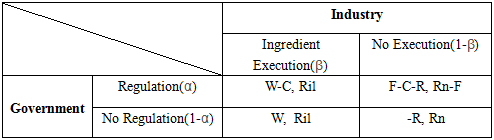
\includegraphics[width=0.5\columnwidth]{figure/result.png}
\label{table:2}
\caption{Table to test captions and labels}
\end{table}
\end{center}

Leveraging all variables we have defined, we could get the Expectation value of government:

\[
E_{il} = \alpha\beta(W-C) + \alpha(1-\beta)(F-C-R) + (1-\alpha)\beta W + (1-\alpha)(1-\beta)R
\]

Analogously, the Expectation value of Industry:

\[
E_c = \alpha\beta R_{il} + \alpha(1-\beta)(R_n-F) + (1-\alpha)\beta R_{il} + (1-\alpha)(1-\beta)R_n
\]

According to the \cite{chenlihong} analysis, we calculate the equilibrium solution for this Game Theory Model, 
and then we get optimal response functions for each entities (Government and Industry).

\begin{equation}
\alpha = \left\{
\begin{array}{ll}
0 & \text{if} \quad \beta > \frac{F-C}{F} \\
\lbrack 0, 1 \rbrack & \text{if} \quad \beta = \frac{F-C}{F} \\
1 & \text{if} \quad \beta < \frac{F-C}{F} \\
\end{array}
\right.
\end{equation}

\begin{equation}
\beta = \left\{
\begin{array}{ll}
0 & \text{if} \quad \alpha < \frac{R_n-R_{il}}{F} \\
\lbrack 0, 1 \rbrack & \text{if} \quad \alpha = \frac{R_n-R_{il}}{F} \\
1 & \text{if} \quad \alpha > \frac{R_n-R_{il}}{F} \\
\end{array}
\right.
\end{equation}


The intersection of two response functions is the mixed Nash equilibrium of the government regulation 
during the execution of Ingredient List. Finally we get the unique deterministic solution, that is 

\[
\alpha^* = \frac{R_n - R_{il}}{F}
\]
\[
\beta^* =  \frac{F - C}{F}
\]

The result illustrates that the Government is intended to regulation the Industries at the probability of $\alpha^*$, 
and the Industry execute Ingredient List at the probability of $\beta^*$, none of them should not 
change this balance state unilaterally, otherwise one of their profits could be damaged.
 
\subsection{Ecosystem of Recycling}
%Maybe picture of this system, if space is required.
% source: Exploring e-waste management systems in the United States
Kahhat et al. proposed a ``deposit-refund system ``~\cite{kahhat2008exploring} for the successful collection and 
recycling of e-waste. In this economic system the consumer has to 
``pay a deposit before purchase, a variable portion of which is returned when turned in at the end-of-life``~\cite{plambeck2009effects}. 
The interest collected by this deposit will compensate for overhead costs such as transportation 
and storage fees of recycling-companies. Moreover, as the returned deposit can vary, 
recycling companies with better recycling processes, can offer a higher return to consumers, 
as they will still gain revenue for the resources in recycled products. 
This system does not only ensure the return of e-waste by consumers, 
but also favors companies, who can recycle more effectively.

However, one huge downside of this system is the requirement to track to-be-sold devices, 
as the deposit is linked to the device. 
Another weakness of Kahhats et al.'s system~\cite{kahhat2008exploring} is that, a company alone would not 
be able to recycle a product completely - however, recycling companies could negate this 
by selling partly recycled products to each other. The specialized companies, which would 
be possible by the ingredient list, would allow this selling process.

With our solution of an ingredient list for all released devices those problems could be alleviated. We would eliminate the deposit 
(and with that the tracking) and merely collect additional tax from Industries who generate the electronics. 
Moreover, consumers will be able to sell their e-waste to recycling companies refunding their tax payment in the process. 
Another important advantage of the ingredient list is that, recycling companies know the 
contents of a device and as such could concentrate on specific recycling processes. 

With the collected tax the government could support the establishment of recycling companies 
and in general the ecosystem of recycling dynamically. This offers huge flexibility, which 
is required in the area of electronics, as this market is an ever changing one. With the 
release of ingredient lists, the government can determine, which resources will be needed 
for production and as a result for recycling. Thus, the government can subsidize effectively and visionary.

To sum up, the ingredient list could eliminate critical weaknesses of Kahhat et al.'s system, 
while also offering new possibilities.

\begin{center}
\begin{table}[!htbp]
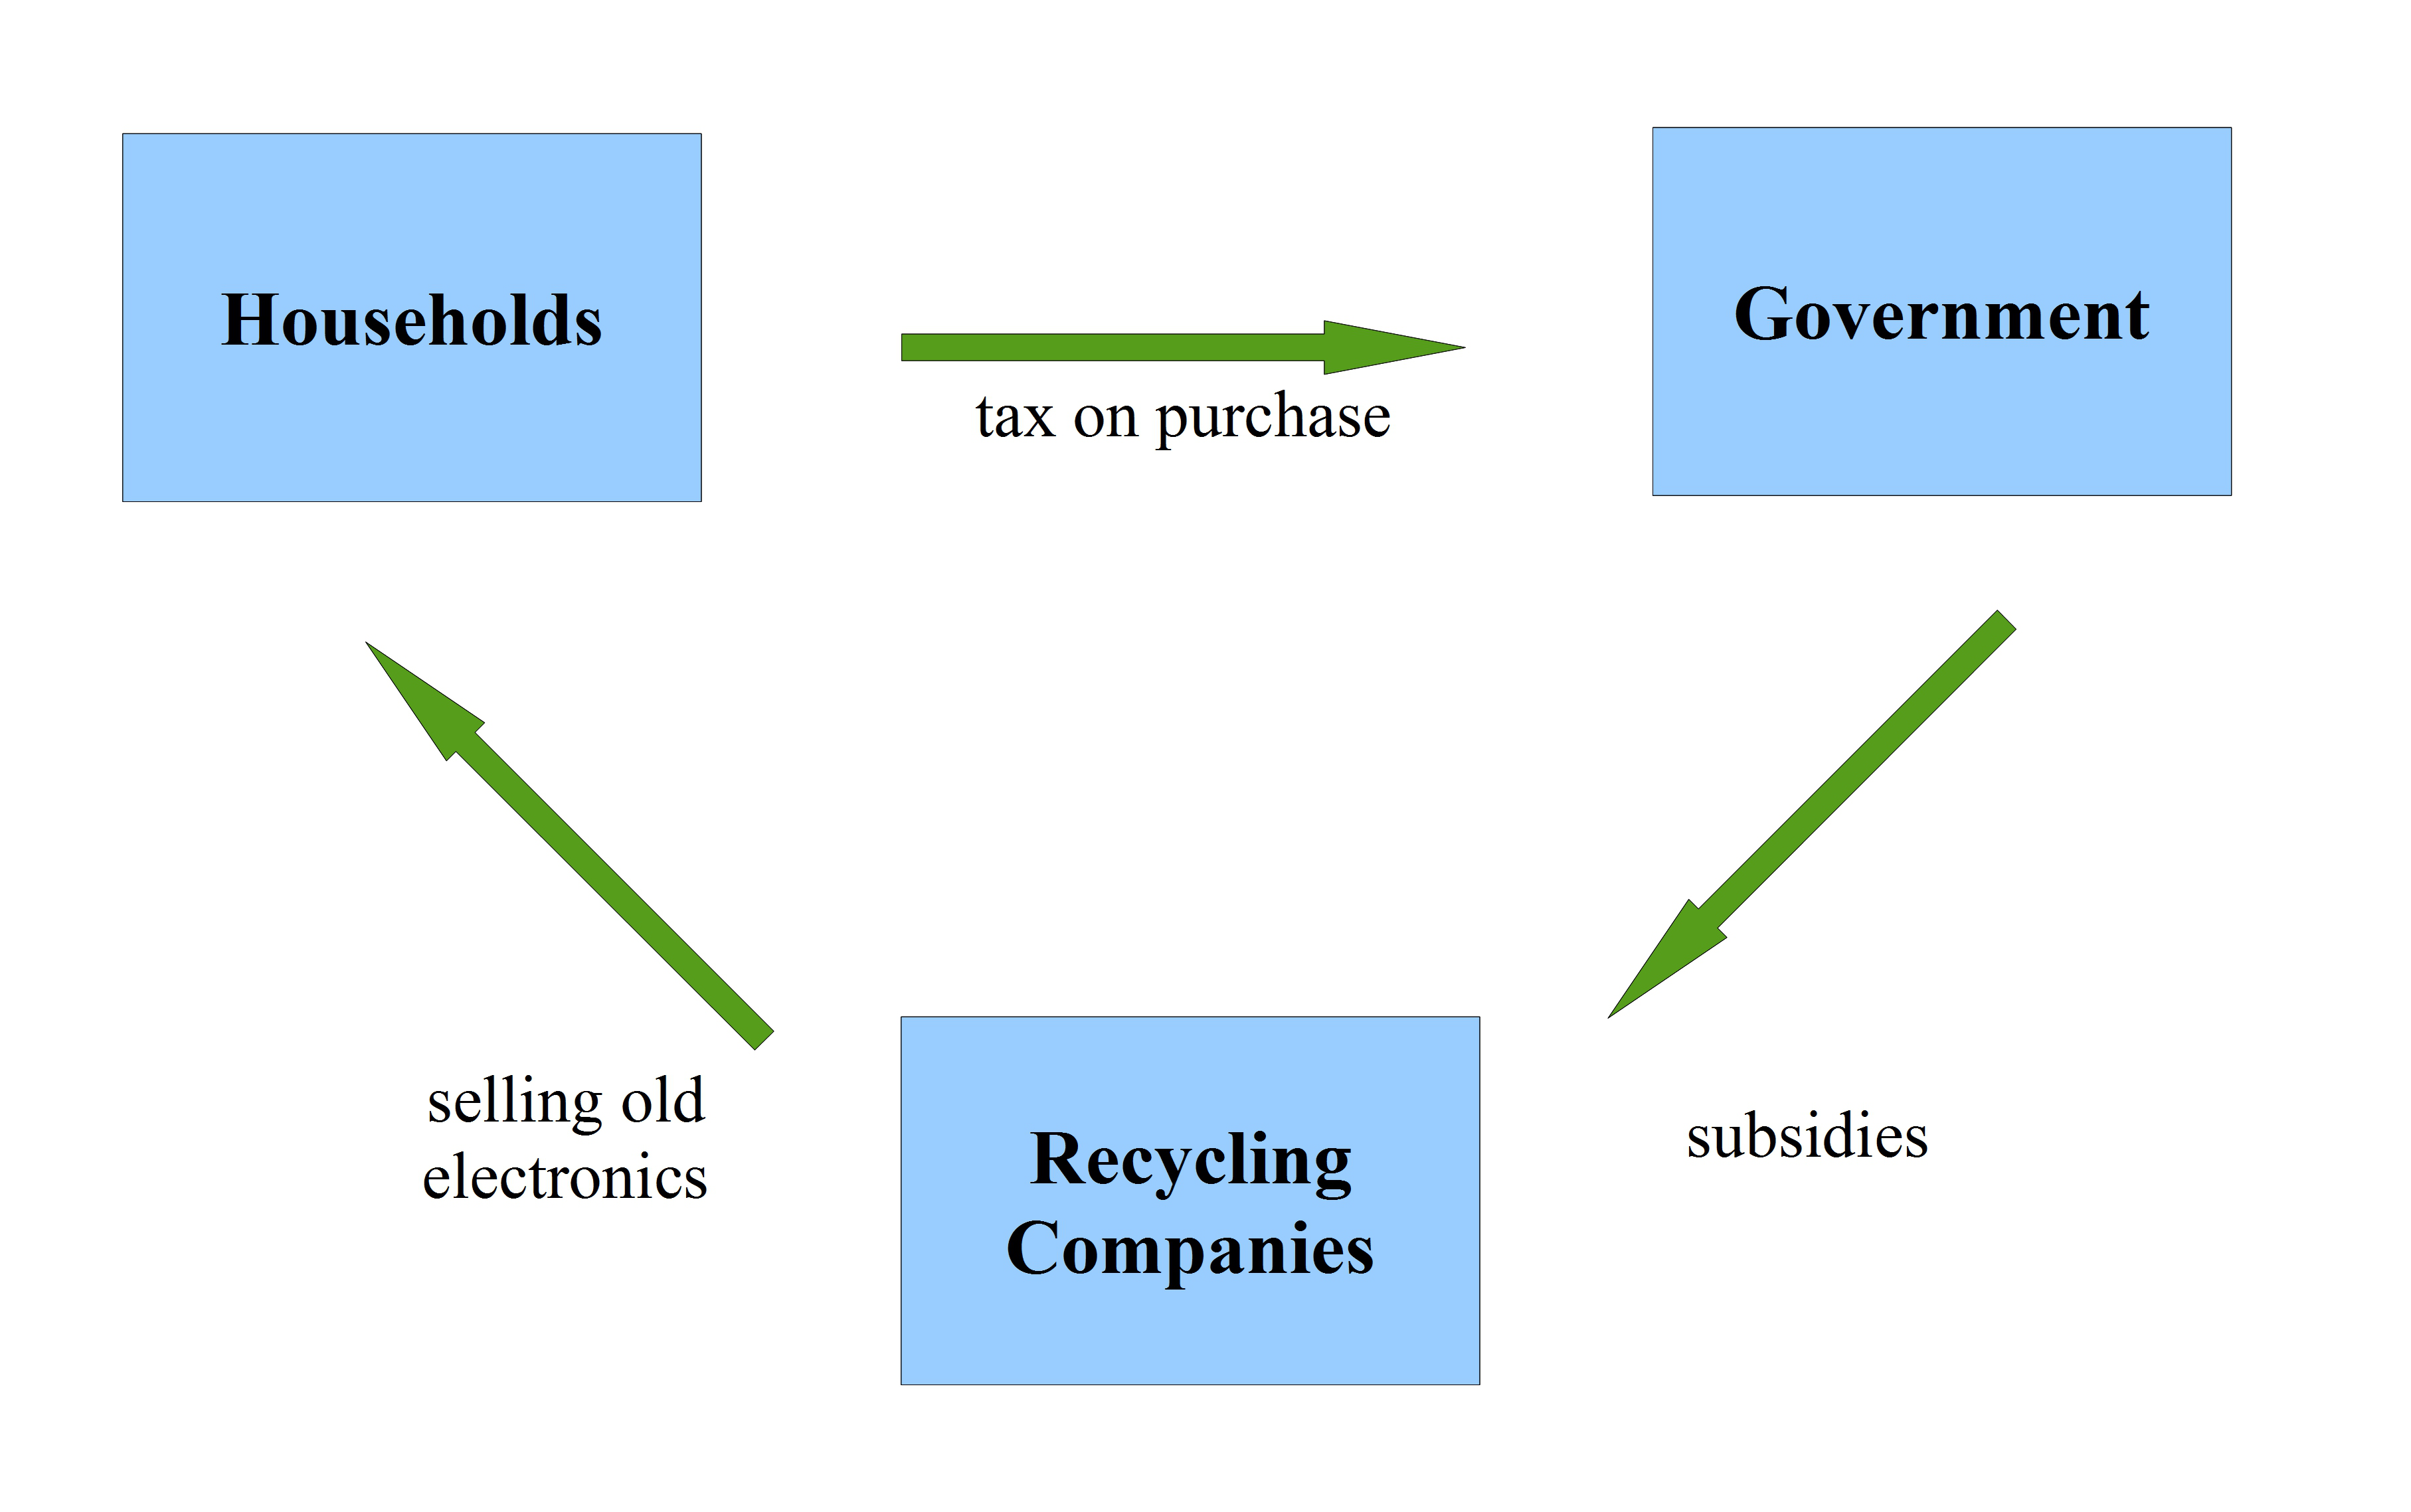
\includegraphics[width=0.5\columnwidth]{figure/cashflow.png}
\label{table:2}
\caption{Cashflow of this system}
\end{table}
\end{center}


\label{applications}
% Expected Problems
\section{Challenges}
% How to get the precise numbers
At first, many producers of electronics may struggle to fulfill this law when their products contain parts delivered by other companies. It would take some time for all the producers to prepare the exact contents of their products. This may increase the price of the product, either because the producer has additional expenses for this or because they just might not do it if the market is too small.\\
% how precise should you be VS how precise can you be?
To be as precise as possible is very important for this approach, especially when the devices are very small and the components contain only grams or milligrams of certain declarable substances. The wanted precision might not always match a feasible one. The determination of the precision of the declaration could be very difficult and therefore has to be explored with care.\\
% what are the ingredients
A disadvantage of this system could concern importers who import non-labeled electronics which weren't originally designed for the European market. It would be the importers' duty to label it himself but mostly this is non-trivial or even impossible. The penalty the importer had to pay would increase the final price for the consumer which is bad for both the consumer and the economy. This problem will persist during the enrollment of this law but may fade with time when producers have caught up.\\
% cheating
One may argue also that it's quite complex to verify the lists the company\'s made and to control the implementing manufacturers. This is because of the volume of devices to control. This problem increases when financial benefits are tied to the contents of these lists although we have put forward a Game Theory. To work out a better solution to this is the task of the corresponding government.
The problems of this approach arise primarily from the context where it is implemented (see \ref{applications}).
% Outlook/future work
\section{Outlook}
As our proposed system of a ingredient list for electronic equipment and devices is only a theoretical construct, as next step it is necessary to test it under real conditions. It is important to find out the practicability of the mapping of food related ingredient lists on electronical related ones. This largely depends on the application and has to be evaluated for every specific use case.\\
\\
In general, more application models can be developed, which also could require different specifications of the ingredients list. For example the sorting of the list may be necessary to adjust: If the emphasize is on toxic materials, the order of the ingredients should be oriented towards this criteria instead of the weight of all used materials. Is the focus is on the special rare materials in order to boost their recycling and so save resources, it is more intuitive to give them a higher priority in the listing of ingredients. Also further other questions can appear: Is an extended labeling of the grade of toxicity necessary instead of just marking all toxic materials in the same way? What else has to be integrated on the ingredient lists (e.g. e-plastic)? Where are the limits of the system (potential need of labeling all components with a ingredient list for partly recycling/resale)?\\
\\
It is also important to evaluate all effects of such a list as our proposed one. Potential influences on different several aspects has to be considered and analyzed one by one. For example there could be negative impacts on the economy: The list can be misconceived by end-consumers and lead to a significant decrease in consumption. Or the establishment of our ingredient list could lead to a disadvantage of the European market against markets, which do not need to fulfill their requirements. Against that, our list could also rise the awareness of the public to recycle. In general, all advantages of our system have to be evaluated in reality, so they can be weight up to negative side effects and disadvantages.\\
\\
We think, our proposed ingredient list holds great potential. It provides a measuring system for e-waste, can raise general awareness in the consumers' mind and so on. It provides the basis for further laws regarding the e-waste problem. This also includes to identify and distribute responsibilities to the different layers of EU government, organizations, producer and the consumer for both evaluating the ingredient list itself as well as developing and executing further rules based on the ingredient list.\\
If the latter once performed, then it is possible to draw comparisons between the resulting system and the e-waste managing systems mentioned in our related work section (see \ref{relatedwork}). Moreover, it is possible to think about a way how these systems can be combined. Therefore, it is necessary to identify all benefits of the existing systems, which would have gone beyond the scope of this work.

\bibliography{acmart} % add or remove the .bib file extension if \cite{bla} does not work for you
\bibliographystyle{ACM-Reference-Format} % add or remove the .bst file extension if \cite{bla} does not work for you

\end{document}
